\documentclass[12pt, spanish]{article}
\usepackage[spanish]{babel}
\selectlanguage{spanish}
%\usepackage{natbib}
\usepackage{url}
\usepackage[utf8x]{inputenc}
\usepackage{graphicx}
\graphicspath{{images/}}
\usepackage{parskip}
\usepackage{fancyhdr}
\usepackage{vmargin}
\usepackage{multirow}
\usepackage{float}
\usepackage{chngpage}

\usepackage{amsfonts}

\usepackage{subcaption}

\usepackage{hyperref}
\usepackage[
    type={CC},
    modifier={by-nc-sa},
    version={4.0},
]{doclicense}

\hypersetup{
    colorlinks=true,
    linkcolor=blue,
    filecolor=magenta,
    urlcolor=cyan,
}

% para codigo
\usepackage{listings}
\usepackage{xcolor}



%% configuración de listings

\definecolor{listing-background}{HTML}{F7F7F7}
\definecolor{listing-rule}{HTML}{B3B2B3}
\definecolor{listing-numbers}{HTML}{B3B2B3}
\definecolor{listing-text-color}{HTML}{000000}
\definecolor{listing-keyword}{HTML}{435489}
\definecolor{listing-identifier}{HTML}{435489}
\definecolor{listing-string}{HTML}{00999A}
\definecolor{listing-comment}{HTML}{8E8E8E}
\definecolor{listing-javadoc-comment}{HTML}{006CA9}

\lstdefinestyle{eisvogel_listing_style}{
  language         = c++,
%$if(listings-disable-line-numbers)$
%  xleftmargin      = 0.6em,
%  framexleftmargin = 0.4em,
%$else$
  numbers          = left,
  xleftmargin      = 0em,
 framexleftmargin = 0em,
%$endif$
  backgroundcolor  = \color{listing-background},
  basicstyle       = \color{listing-text-color}\small\ttfamily{}\linespread{1.15}, % print whole listing small
  breaklines       = true,
  frame            = single,
  framesep         = 0.19em,
  rulecolor        = \color{listing-rule},
  frameround       = ffff,
  tabsize          = 4,
  numberstyle      = \color{listing-numbers},
  aboveskip        = 1.0em,
  belowskip        = 0.1em,
  abovecaptionskip = 0em,
  belowcaptionskip = 1.0em,
  keywordstyle     = \color{listing-keyword}\bfseries,
  classoffset      = 0,
  sensitive        = true,
  identifierstyle  = \color{listing-identifier},
  commentstyle     = \color{listing-comment},
  morecomment      = [s][\color{listing-javadoc-comment}]{/**}{*/},
  stringstyle      = \color{listing-string},
  showstringspaces = false,
  escapeinside     = {/*@}{@*/}, % Allow LaTeX inside these special comments
  literate         =
  {á}{{\'a}}1 {é}{{\'e}}1 {í}{{\'i}}1 {ó}{{\'o}}1 {ú}{{\'u}}1
  {Á}{{\'A}}1 {É}{{\'E}}1 {Í}{{\'I}}1 {Ó}{{\'O}}1 {Ú}{{\'U}}1
  {à}{{\`a}}1 {è}{{\'e}}1 {ì}{{\`i}}1 {ò}{{\`o}}1 {ù}{{\`u}}1
  {À}{{\`A}}1 {È}{{\'E}}1 {Ì}{{\`I}}1 {Ò}{{\`O}}1 {Ù}{{\`U}}1
  {ä}{{\"a}}1 {ë}{{\"e}}1 {ï}{{\"i}}1 {ö}{{\"o}}1 {ü}{{\"u}}1
  {Ä}{{\"A}}1 {Ë}{{\"E}}1 {Ï}{{\"I}}1 {Ö}{{\"O}}1 {Ü}{{\"U}}1
  {â}{{\^a}}1 {ê}{{\^e}}1 {î}{{\^i}}1 {ô}{{\^o}}1 {û}{{\^u}}1
  {Â}{{\^A}}1 {Ê}{{\^E}}1 {Î}{{\^I}}1 {Ô}{{\^O}}1 {Û}{{\^U}}1
  {œ}{{\oe}}1 {Œ}{{\OE}}1 {æ}{{\ae}}1 {Æ}{{\AE}}1 {ß}{{\ss}}1
  {ç}{{\c c}}1 {Ç}{{\c C}}1 {ø}{{\o}}1 {å}{{\r a}}1 {Å}{{\r A}}1
  {€}{{\EUR}}1 {£}{{\pounds}}1 {«}{{\guillemotleft}}1
  {»}{{\guillemotright}}1 {ñ}{{\~n}}1 {Ñ}{{\~N}}1 {¿}{{?`}}1
  {…}{{\ldots}}1 {≥}{{>=}}1 {≤}{{<=}}1 {„}{{\glqq}}1 {“}{{\grqq}}1
  {”}{{''}}1
}
\lstset{style=eisvogel_listing_style}


\usepackage[default]{sourcesanspro}

\setmarginsrb{2 cm}{1 cm}{2 cm}{2 cm}{1 cm}{1.5 cm}{1 cm}{1.5 cm}

\title{Ejercicio 2:\\
Sistema de inventario.\hspace{0.05cm} }
\author{Antonio David Villegas Yeguas}
\date{\today}

\renewcommand*\contentsname{hola}

\makeatletter
\let\thetitle\@title
\let\theauthor\@author
\let\thedate\@date
\makeatother

\pagestyle{fancy}
\fancyhf{}
\rhead{\theauthor}
\lhead{\thetitle}
\cfoot{\thepage}

\begin{document}

%%%%%%%%%%%%%%%%%%%%%%%%%%%%%%%%%%%%%%%%%%%%%%%%%%%%%%%%%%%%%%%%%%%%%%%%%%%%%%%%%%%%%%%%%

\begin{titlepage}
    \centering
    \vspace*{0.3 cm}
    
\includegraphics[scale = 0.50]{ugr.png}\\[0.7 cm]
    %\textsc{\LARGE Universidad de Granada}\\[2.0 cm]
    \textsc{\large 4º CSI 2020/21 - Grupo 1}\\[0.5 cm]
    \textsc{\large Grado en Ingeniería Informática}\\[0.5 cm]
    \rule{\linewidth}{0.2 mm} \\[0.2 cm]
    { \huge \bfseries \thetitle}\\
    \rule{\linewidth}{0.2 mm} \\[1 cm]

    \begin{minipage}{0.4\textwidth}
        \begin{flushleft} \large
            \emph{Autor:}\\
            \theauthor\\
			 \emph{DNI:}\\
            77021623-M
            \end{flushleft}
            \end{minipage}~
            \begin{minipage}{0.4\textwidth}
            \begin{flushright} \large
            \emph{Asignatura: \\
            Simulación de Sistemas}   \\
            \emph{Correo:}\\
            advy99@correo.ugr.es
        \end{flushright}
    \end{minipage}\\[0.5cm]

    {\large \thedate}\\[0.5cm]
    %{\url{https://github.com/advy99/AA/}}
    {\doclicenseThis}

    \vfill

\end{titlepage}

%%%%%%%%%%%%%%%%%%%%%%%%%%%%%%%%%%%%%%%%%%%%%%%%%%%%%%%%%%%%%%%%%%%%%%%%%%%%%%%%%%%%%%%%%

\tableofcontents
\pagebreak

%%%%%%%%%%%%%%%%%%%%%%%%%%%%%%%%%%%%%%%%%%%%%%%%%%%%%%%%%%%%%%%%%%%%%%%%%%%%%%%%%%%%%%%%%


\section*{Introducción}

Para este ejercicio se nos pide simular el funcionamiento de un sistema de inventario que venderá un único objeto. Para implementar este sismtema utilizaremos un modelo discreto y en este documento explicaré como se ha implementado, así como los sucesos, el grafo de sucesos, las variables de interés y experimentación.

\section{Descripción del problema}

El problema se basa en simular el trabajo de una compañia que vende un único producto y se quiere decidir cuantos items mantener en inventario durante una cierta cantidad de meses.

Los tiempos enter demanda del producto serán variables aleatorias independientes e identicamente distribuidas, exponenciales con media 0.1 por mes, es decir, una demanda cada tres días de media. El tamaño de las demandas es una variable aleatoria con la siguiente distribución:

\begin{itemize}
	\item $D = 1$ con probabilidad $1/6$
	\item $D = 2$ con probabilidad $1/3$
	\item $D = 3$ con probabilidad $1/3$
	\item $D = 4$ con probabilidad $1/6$
\end{itemize}


Al inicio de cada més la compañia decidirá cuantos objetos pedir, utilizando la siguiente política estacionaria (s, S):

\begin{itemize}
	\item $Z = S - I$ si $I < s$
	\item $Z = 0$ si $I \geq s$
\end{itemize}

Donde I es el nivel de inventario antes de hacer el pedido.

Tras saber cuantos items pedir, el costo será de $K + iZ$, donde $K = 32$ y será el costo de hacer el pedido e $i = 3$ y se trata de el costo por item. Si Z es cero, no se gastará nada.

Cuando se hace el pedido este llegará en un periodo que será una variable aleatoria uniformemente distribuida entre 0.5 y 1 mes.

Además del costo de pedido, existe el costo de mantenimiento y de déficit.

El costo medio de mantenimiento de los items para los n meses es:

\[ h \frac{\int_0^n I^+ (t) dt}{n} \]

Donde $h = 1$ por item y por mes, y $\frac{\int_0^n I^+ (t) dt}{n}$ el numero medio real de items en el inventario. Este coste tiene en cuenta alguileres, seguros, tasas, etc.

El costo medio de déficit para los n meses es:

\[ \pi \frac{\int_0^n I^- (t) dt}{n} \]

Donde $\pi = 5$ por item y por mes, y $\frac{\int_0^n I^- (t) dt}{n}$ el numero medio de items vendidos pero no vendidos. Esto incluye pérdidas de confianza de clientes entre otros.

En concreto a nosotros se nos pide trabajar con un sistema donde $I(0) = 60$, es decir al inicio tendremos 60 items y no habrá ningún pedido en curso. También nos piden que la simulación se haga para 10 años completos, en nuestra unidad de trabajo, 120 meses.


\section{Planteamiento de la solución al problema}

De cara a resolver el problema he implementado una clase en C++ llamada \texttt{SistemaInventario} que contendrá todas las variables y métodos necesarios para simular el sistema. De esta forma podremos ampliar y modificar el funcionamiento del sistema con mucha facilidad.

\subsection{Variables de interes}

Como variables de interes entontramos tres tipos:

\begin{enumerate}
	\item Variables del problema (independientes a la implementación):
		\begin{itemize}
			\item \texttt{nivel}: Nivel de inventario.
			\item \texttt{pedido}: Número de items a pedir en un mes.
			\item \texttt{costo_hacer_pedido}: Variable K en la descripción del problema.
			\item \texttt{costo_por_unidad}: Variable i en la descripción del problema.
			\item \texttt{s_pequena}: Junto a \texttt{s_grande}, política de pedido.
			\item \texttt{s_grande}: Junto a \texttt{s_pequena}, política de pedido.
		\end{itemize}

	\item Variables estadísticas (para realizar el informe):
		\begin{itemize}
			\item \texttt{acum_mas}: Acumulador del area bajo $I^+(t)$.
			\item \texttt{acum_menos}: Acumulador del area bajo $I^+(t)$.
			\item \texttt{acum_pedido}: Acumulador del costo del pedido.
		\end{itemize}

	\item Variables de la implementación del sistema:
		\begin{itemize}
			\item \texttt{reloj}: Contador del reloj sobre el mes actual para realizar los sucesos.
			\item \texttt{parar}: Booleano que nos dice cuando hemos llegado al fin de la simulación.
			\item \texttt{informe}: Vector donde almacenaremos las variables estadísticas para generar el informe entre simulaciones.
			\item \texttt{l_suc}: Lista de sucesos.
		\end{itemize}
\end{enumerate}

La lista de sucesos será una lista que siempre tendremos ordenada, y contendrá elementos de la siguiente estructura:

\begin{lstlisting}
typedef struct {
	Suceso suceso;
	double tiempo;
} suc;
\end{lstlisting}

En la que almacenaremos el tipo de suceso y el lugar de tiempo donde se dará dicho suceso. Esta lista estará siempre ordenada y los posibles sucesos los he definido de la siguiente forma:

\begin{lstlisting}
enum class Suceso {SUCESO_DEMANDA, SUCESO_EVALUACION_INVENTARIO, SUCESO_LLEGADA_PEDIDO, SUCESO_FIN_SIMULACION};
\end{lstlisting}

Estos sucesos representan lo siguiente:

\begin{itemize}
	\item \texttt{SUCESO\_DEMANDA}: Se produce una demanda de items en el sistema.
	\item \texttt{SUCESO\_EVALUACION\_INVENTARIO}: Se produce una evaluación del inventario de cara a pedir más items si es necesario.
	\item \texttt{SUCESO\_LLEGADA\_PEDIDO}: Ha llegado un pedido realizado en la evaluación del inventario.
	\item \texttt{SUCESO\_FIN\_SIMULACION}: Se ha llegado al final de la simulación.
\end{itemize}

De esta forma tendremos una función \texttt{insertar_lsuc} para insertar un suceso en la lista de sucesos, a la que se le pasan dos parámetros, el tipo de suceso del enum \texttt{Suceso} y el tiempo donde corresponde dicho suceso. Esta función insertará dicho suceso y ordenará la lista de sucesos de cara a que cada uno se ejecute en su correspondiente orden.

\subsection{Inicialización del sistema}


\subsection{Sucesos}


\subsection{Grafo de sucesos}

\begin{figure}[H]
  \centering
   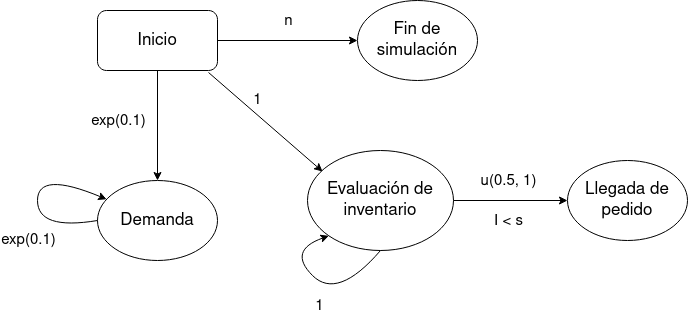
\includegraphics[width=\textwidth]{grafo_sucesos_original.png}
	\caption{Grafo de estados del sistema original.}
\end{figure}


\subsection{Primera modificación}

\begin{figure}[H]
  \centering
   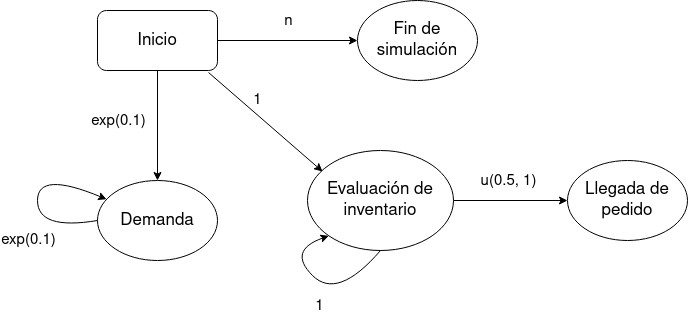
\includegraphics[width=\textwidth]{grafo_sucesos_mod1.png}
	\caption{Grafo de estados del sistema con la primera modificación.}
\end{figure}


\subsection{Segunda modificación}

\begin{figure}[H]
  \centering
   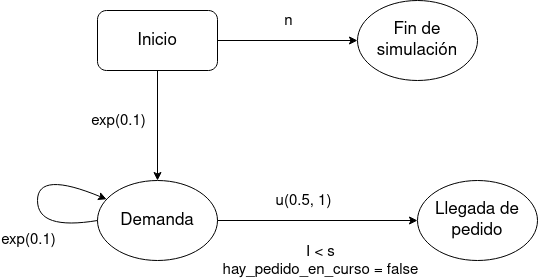
\includegraphics[width=\textwidth]{grafo_sucesos_mod2.png}
	\caption{Grafo de estados del sistema con la segunda modificación.}
\end{figure}




\section{Experimentos}


\subsection{Sistema original}





\begin{table}[H]
\resizebox{\textwidth}{!}{%
\begin{tabular}{|c|c|c|c|c|c|}
\hline
\textbf{Modificacion} & \textbf{Política} & \textbf{Costo total} & \textbf{Costo de pedido} & \textbf{Costo de mantenimiento} & \textbf{Costo de déficit} \\ \hline
0                     & (0, 40)           & 146.069              & 87.8906                  & 5.818                           & 52.3599                   \\ \hline
0                     & (0, 60)           & 135.798              & 84.3302                  & 12.9894                         & 38.4786                   \\ \hline
0                     & (0, 80)           & 134.081              & 82.3902                  & 21.2874                         & 30.4028                   \\ \hline
0                     & (0, 100)          & 136.563              & 81.2397                  & 30.1069                         & 25.2168                   \\ \hline
0                     & (20, 40)          & 124.954              & 97.5676                  & 9.12249                         & 18.2638                   \\ \hline
0                     & (20, 60)          & 118.946              & 88.5286                  & 17.4971                         & 12.9206                   \\ \hline
0                     & (20, 80)          & 121.262              & 84.8902                  & 26.875                          & 9.49655                   \\ \hline
0                     & (20, 100)         & 126.882              & 82.9485                  & 36.4578                         & 7.4752                    \\ \hline
0                     & (40, 60)          & 125.698              & 98.3373                  & 25.5159                         & 1.84459                   \\ \hline
0                     & (40, 80)          & 125.475              & 89.1619                  & 34.9504                         & 1.36322                   \\ \hline
0                     & (40, 100)         & 131.512              & 85.5084                  & 44.9817                         & 1.02162                   \\ \hline
0                     & (60, 80)          & 143.831              & 98.8766                  & 44.8827                         & 0.0718687                 \\ \hline
0                     & (60, 100)         & 144.145              & 89.6238                  & 54.4677                         & 0.0530768                 \\ \hline
\end{tabular}
}
\end{table}

La mejor politica con la modificación 0 es la política: (20, 60) con un costo total de 118.946



\subsection{Primera modificación}






\begin{table}[H]
\resizebox{\textwidth}{!}{%
\begin{tabular}{|c|c|c|c|c|c|}
\hline
\textbf{Modificacion} & \textbf{Política} & \textbf{Costo total} & \textbf{Costo de pedido} & \textbf{Costo de mantenimiento} & \textbf{Costo de déficit} \\ \hline
1    &    (0, 40)    &    135.554    &    106.013    &    29.0519    &    0.48888                  \\ \hline
1    &    (0, 60)    &    135.555    &    106.012    &    29.0596    &    0.483654                  \\ \hline
1    &    (0, 80)    &    135.555    &    106.019    &    29.0522    &    0.483913                  \\ \hline
1    &    (0, 100)    &    135.559    &    106.015    &    29.0598    &    0.48414                 \\ \hline
1    &    (20, 40)    &    135.547    &    105.99    &    29.0676    &    0.48974                 \\ \hline
1    &    (20, 60)    &    135.548    &    105.999    &    29.0621    &    0.487301                 \\ \hline
1    &    (20, 80)    &    135.576    &    106.038    &    29.0457    &    0.492535                 \\ \hline
1    &    (20, 100)    &    135.541    &    105.995    &    29.0598    &    0.487079                 \\ \hline
1    &    (40, 60)    &    135.509    &    105.955    &    29.0734    &    0.480824                 \\ \hline
1    &    (40, 80)    &    135.56    &    106.014    &    29.0521    &    0.493923                 \\ \hline
1    &    (40, 100)    &    135.555    &    106.006    &    29.0538    &    0.495418                 \\ \hline
1    &    (60, 80)    &    135.552    &    106.005    &    29.0624    &    0.485406                 \\ \hline
1    &    (60, 100)    &    135.528    &    105.975    &    29.0676    &    0.485268                 \\ \hline
\end{tabular}
}
\end{table}

La mejor politica con la modificación 1 es la política: (40, 60) con un costo total de 135.509



\subsection{Segunda modificación}





\begin{table}[H]
\resizebox{\textwidth}{!}{%
\begin{tabular}{|c|c|c|c|c|c|}
\hline
\textbf{Modificacion} & \textbf{Política} & \textbf{Costo total} & \textbf{Costo de pedido} & \textbf{Costo de mantenimiento} & \textbf{Costo de déficit} \\ \hline
2                     & (0,40)            & 125.858              & 92.8172                  & 7.37356                         & 25.6674                   \\ \hline
2                     & (0,60)            & 119.998              & 87.0855                  & 15.5162                         & 17.3962                   \\ \hline
2                     & (0,80)            & 121.88               & 84.2024                  & 24.4991                         & 13.179                    \\ \hline
2                     & (0,100)           & 127.009              & 82.5815                  & 33.8                            & 10.6271                   \\ \hline
2                     & (20,40)           & 124.725              & 106.047                  & 11.5856                         & 7.09213                   \\ \hline
2                     & (20,60)           & 117.751              & 93.4749                  & 22.2932                         & 1.98309                   \\ \hline
2                     & (20,80)           & 121.021              & 87.6426                  & 32.0481                         & 1.32992                   \\ \hline
2                     & (20,100)          & 127.622              & 84.7731                  & 41.842                          & 1.0068                    \\ \hline
2                     & (40,60)           & 136.932              & 106.743                  & 29.928                          & 0.261081                  \\ \hline
2                     & (40,80)           & 135.806              & 94.1011                  & 41.6824                         & 0.0224374                 \\ \hline
2                     & (40,100)          & 139.864              & 88.2214                  & 51.6284                         & 0.0146204                 \\ \hline
2                     & (60,80)           & 157.186              & 107.487                  & 49.6953                         & 0.00380315                \\ \hline
2                     & (60,100)          & 156.27               & 94.6649                  & 61.6051                         & 5.55898e-05               \\ \hline
\end{tabular}
}
\end{table}

La mejor politica con la modificación 2 es la política: (20, 60) con un costo total de 117.751








% \begin{thebibliography}{9}
%
%
% \end{thebibliography}

\end{document}
